\documentclass[11pt]{exam}
\usepackage[utf8]{inputenc}
\usepackage[a4paper,top=2cm,left=2cm,right=2cm,bottom=2cm]{geometry}
\usepackage{import}
\usepackage[T1]{fontenc}
\usepackage[german,ngerman]{babel}
\usepackage[table]{xcolor}
\usepackage{amsthm, esvect}
\usepackage{mathtools}
\RequirePackage{amssymb, amsfonts, amsmath, latexsym, verbatim, xspace}
\usepackage{systeme}
\usepackage{multicol}
\usepackage{multirow}
\usepackage{framed}
\usepackage{array}
\usepackage{ragged2e}
\usepackage{graphicx}
\usepackage{pdflscape}
\usepackage{epstopdf}
\usepackage{booktabs}
\usepackage{pdfpages}
\usepackage{float} % Allows putting an [H] in \begin{figure} to specify the exact location of the figure
\usepackage{wrapfig} % Allows in-line images such as the example fish picture
\usepackage{tikz, graphicx} % tikz
\usepackage[position=top]{subfig}
\usepackage[bookmarks=true]{hyperref}%Links
\usepackage{enumerate}
\usepackage{enumitem}
\usepackage[german,ruled,vlined,linesnumbered,algosection]{algorithm2e}
\usepackage[labelfont=sf]{caption}
\usepackage{lmodern}
\usepackage{lscape}
\usepackage{tabularx}
\usepackage{systeme}
\usepackage{hhline}
\usepackage{subfiles}
\usepackage{stackengine}
\usepackage{setspace}
\usepackage{MnSymbol}
\usepackage{tcolorbox}
\usepackage{bbm}
\usepackage{url}
\usepackage{xparse}
\usepackage{sectsty}
\usepackage{array}
\usepackage{ragged2e}
\usepackage{listings} %Stellt Code-Snippets sauber dar

% definiert die Sprache
\selectlanguage{German}

% add command for different dates in Swiss fashion
\newcommand{\monthwordlong}[1]{\ifcase#1 \or Januar\or Februar\or März\or April\or Mai\or Juni\or Juli\or August\or September\or Oktober\or November\or Dezember\fi}
\newcommand{\monthwordshort}[1]{\ifcase#1\or Jan\or Feb\or Mar\or Apr\or Mai\or Jun\or Jul\or Aug\or Sept\or Okt\or Nov\or Dez\fi}
\newcommand{\datelong}{\number\day.\:\monthwordlong{\the\month}\:\number\year}
\newcommand{\dateshort}{\number\day.\:\monthwordshort{\the\month}\:\number\year}

% define color of links inside a text
\definecolor{linkblue}{RGB}{0, 0, 80}
\definecolor{plotblue}{RGB}{100, 100, 255}
\definecolor{myblue}{RGB}{8,164,214}
\definecolor{myred}{RGB}{143,42,41}
\definecolor{forestgreen}{RGB}{34,139,34}
\definecolor{highdive}{RGB}{10,169,194}
\definecolor{charcoal}{RGB}{74,74,74}
\hypersetup{
	colorlinks=true,
	linkcolor=linkblue,
	filecolor=magenta,
	urlcolor=plotblue,
	citecolor=linkblue,
	pdfpagemode=FullScreen,
}


\lstdefinestyle{mystyle}{ % definiert den style des Code-Snippets
	%backgroundcolor=\color{backcolour},
	%commentstyle=\color{codegreen},
	%keywordstyle=\color{magenta},
	%numberstyle=\tiny\color{codegray},
	%stringstyle=\color{codepurple},
	basicstyle=\ttfamily\footnotesize,
	breakatwhitespace=false,
	breaklines=true,
	captionpos=b,
	keepspaces=true,
	%numbers=left,
	%numbersep=5pt,
	showspaces=false,
	showstringspaces=false,
	showtabs=false,
	tabsize=4
}
\lstset{style=mystyle}
\qformat{\Large\textbf{Aufgabe \thequestion\hfill\thepoints}}
\newlist{partes}{enumerate}{3}
\setlist[partes]{label=(\alph*)}
\newcommand{\parte}{\item}
\newlist{subpartes}{enumerate}{3}
\setlist[subpartes]{label=\roman*)}
\newcommand{\subparte}{\item}
\setlist[enumerate,1]{%(
	leftmargin=*, itemsep=12pt, label={\textbf{\arabic*.)}}}
\newcommand\answerbox{%%
	\fbox{\rule{2in}{0pt}\rule[-0.1ex]{0pt}{4ex}}}
\pointpoints{Punkt}{Punkte}
\hqword{Frage:}
\hpword{Mögliche Punkte:}
\hsword{Erreicht:}
\htword{Total}
\renewcommand*\half{.5}
\renewcommand{\solutiontitle}{\noindent\textbf{Lösung:}\par\noindent}

% Graphed boxes
\newcommand{\karos}[2]{
  \begin{tikzpicture}
    \draw[step=0.4cm,color=cyan,dotted] (0,0) grid (#1 cm ,#2 cm);
  %  \draw((#1)/2 cm,0)--((#1)/2 cm,/#2)/2cm)
  \end{tikzpicture}
}
\usetikzlibrary{arrows, petri, topaths, graphs}
\linespread{1.2} % Line spacing

%=========================================================
\newenvironment{parcols}[1][]{
    \begin{parts}\begin{multicols}{#1}
}{
    \end{multicols}\end{parts}
}
%=========================================================
\newenvironment{itemcols}[1][]{
	\begin{itemize}\begin{multicols}{#1}
		}{
	\end{multicols}\end{itemize}
}

%=========================================================
\newcommand{\antwort}[1]{
	{\setlength{\textwidth}{\textwidth}\fillwithgrid{#1cm}\vspace{5pt}}
}

%=========================================================
% Karriertes Papier für Antwort MIT OVERLAY
\tcbuselibrary{breakable,skins}
\usetikzlibrary{mindmap,trees}
\newlength\tindent
\setlength{\tindent}{\parindent}
\setlength{\parindent}{0pt}
\setlength{\parskip}{0pt}

\newtcolorbox{gridspace}[1]{%
	enhanced,
	breakable,
	blanker,
	boxrule=0pt,
	left=5mm,
	right=5mm,
	top=5.75mm,
	bottom=0mm,
	boxsep=0pt,
	height=#1cm,
	width=16cm,
	before upper={
		\begingroup
		\setlength{\baselineskip}{5.75mm}
		\setlength{\parskip}{0pt}
		\setlength{\lineskip}{0pt}
		% keep every paragraph on the grid rhythm
		%\everypar{\vspace{0pt}\strut}
		% math formulas shifted by one grid row
		\let\oldbracketopen\[
		\renewcommand{\[}{\vspace{-5mm}\oldbracketopen}
		% Align displayed formulas to the grid
		\setlength{\abovedisplayskip}{0pt}
		\setlength{\belowdisplayskip}{0pt}
		\setlength{\abovedisplayshortskip}{0pt}
		\setlength{\belowdisplayshortskip}{0pt}
		% Enumerate follows the same rhythm
		\setlist[enumerate]{leftmargin=6mm,itemsep=0mm,topsep=0pt,parsep=0pt,partopsep=0pt}
		\setlist[itemize]{leftmargin=6mm,itemsep=10mm,topsep=0pt,parsep=0pt,partopsep=0pt}},
	after upper={
		\endgroup},
	underlay={
		\draw[step=5mm,color=gray!55] (interior.south west) grid (interior.north east);}
}

\pagestyle{headandfoot}
\firstpageheader{}{}{\teacher}
\runningheader{}{}{\teacher}
\firstpagefooter{}{}{Seite \thepage\:von \numpages}
\runningfooter{}{}{Seite \thepage\:von \numpages}
%%
% Math Arrows
%%
\newcommand{\same}{\ensuremath{\Longleftrightarrow}}
\renewcommand{\to}{\ensuremath{\longrightarrow}}
\newcommand{\qsame}{\quad\same\quad}
\newcommand{\dsame}{\ensuremath{:\Leftrightarrow}}
\newcommand{\qdsame}{\quad\dsame\quad}
\newcommand{\ldsame}{\ensuremath{:\Longleftrightarrow}}
\newcommand{\samedef}{\ensuremath{\us {\text{def}} \Leftrightarrow}}
\newcommand{\qsamedef}{\quad\samedef\quad}
\newcommand{\lsamedef}{\ensuremath{\us {\text{def}} \Longleftrightarrow}}
\newcommand{\qlsamedef}{\quad\lsamedef\quad}


%%
% Mengendefinitionen
%%
\newcommand{\M}{\ensuremath{\mathcal{M}}}
\newcommand{\N}{\ensuremath{\mathbb{N}}}
\newcommand{\Z}{\ensuremath{\mathbb{Z}}}
\newcommand{\Q}{\ensuremath{\mathbb{Q}}}
\newcommand{\I}{\ensuremath{\mathbb{I}}}
\newcommand{\R}{\ensuremath{\mathbb{R}}}
\newcommand{\C}{\ensuremath{\mathbb{C}}}
\renewcommand{\S}{\ensuremath{\mathbb{S}}}
\newcommand{\Prim}{\ensuremath{\mathbb{P}}}
\newcommand{\0}{\ensuremath{\emptyset}}
\renewcommand{\Re}{\ensuremath{\operatorname{Re}}}
\renewcommand{\Im}{\ensuremath{\operatorname{Im}}}
\newcommand{\strich}{\ensuremath{\big\vert}}

%%
% Mengenoperation
%%
\renewcommand{\nin}{\not\in}


%%
% Logisches Und und Oder
%%
\newcommand{\sand}{\ensuremath{\; \land \;}}
\newcommand{\sor}{\ensuremath{\; \lor \;}}
\renewcommand{\*}{\ensuremath{\cdot}}
\newcommand{\oder}{\vee}
\newcommand{\n}{\neg}
\newcommand{\und}{\wedge}


%%
% Bei Integral, Summe,... die Grenzen über bzw.
% unter das Zeichen
%%
\renewcommand{\d}[1]{\ensuremath{\operatorname{d}\!{#1}}}
\newcommand{\Sum}{\sum\limits}
\newcommand{\Prod}{\prod\limits}
\newcommand{\Min}{\min\limits}
\newcommand{\Max}{\max\limits}
\newcommand{\Lim}{\lim\limits}
\newcommand{\Inf}{\inf\limits}
\newcommand{\Sup}{\sup\limits}
\newcommand{\Liminf}{\liminf\limits}
\newcommand{\Limsup}{\limsup\limits}
%\renewcommand{\Cup}{\bigcup\limits}
%\renewcommand{\Cap}{\bigcap\limits}
\newcommand{\Otimes}{\bigotimes\limits}
\newcommand{\Oplus}{\bigoplus\limits}


%%
% Arcus Cotangens, Logarithmus
%%
\let\oldsin\sin
\renewcommand{\sin}[1]{\oldsin{\left(#1\right)}}
\let\oldcos\cos
\renewcommand{\cos}[1]{\oldcos{\left(#1\right)}}
\let\oldtan\tan
\renewcommand{\tan}[1]{\oldtan{\left(#1\right)}}
\let\oldarcsin\arcsin
\renewcommand{\arcsin}[1]{\oldarcsin{\left(#1\right)}}
\let\oldarccos\arccos
\renewcommand{\arccos}[1]{\oldarccos{\left(#1\right)}}
\let\oldarctan\arctan
\renewcommand{\arctan}[1]{\oldarctan{\left(#1\right)}}
\let\oldln\ln
\renewcommand{\ln}[1]{\oldln{\left(#1\right)}}
\newcommand{\Log}[2]{\ensuremath{\operatorname{log}_{#1}\left(#2\right)}}
\newcommand{\e}{\operatorname{e}}
\renewcommand{\exp}[1]{\ensuremath{\operatorname{\e}^{#1}}}


%%
% Griechische Buchstaben
%%
\renewcommand{\epsilon}{\ensuremath{\varepsilon}}
\renewcommand{\phi}{\varphi}
\renewcommand{\l}{\lambda}
\renewcommand{\t}{\tau}


%%
% Bezeichnungen
%%
\newcommand{\Rgn}{\R_{>0}} % R grösser Null
\newcommand{\Rad}{\operatorname{Rad}}   % Radikal
\newcommand{\kgV}{\operatorname{kgV}}   % Kleinster gemeinsame Vielfache
\newcommand{\ggT}{\operatorname{ggT}}   % Grösster gemeinsame Teiler
\newcommand{\winkel}{\sphericalangle}          % Winkelsymbol
\DeclarePairedDelimiter\abs{\lvert}{\rvert} % besserer Betrag
\makeatletter
\let\oldabs\abs
\def\abs{\@ifstar{\oldabs}{\oldabs*}}
\makeatother


%%
% Vektorgeometrie
%%
\renewcommand{\v}[1]{\vv{#1}}       % besserer Pfeil über Buchstaben
\renewcommand{\vec}[2]{\begingroup\renewcommand{\arraystretch}{1}\left(\begin{array}{c} #1 \\ #2 \end{array}\right)\endgroup}   % two dimensional vector
\renewcommand{\Vec}[3]{\begingroup\renewcommand{\arraystretch}{1}\left(\begin{array}{c} #1 \\ #2 \\ #3 \end{array}\right)\endgroup}      % three dimensional vector


%%
% Text
%%
\newcommand*{\Ueq}[1]{\mathrel{\mathop{=}\limits_{\text{#1}}}}
\newcommand*{\Oeq}[1]{\mathrel{\stackrel{\text{#1}}{=}}}
\newcommand{\utext}[2]{\underbrace{#1}_{\substack{#2}}}
\newcommand{\otext}[2]{$\overbrace{\textrm{#1}}^{\textrm{#2}}$}
\newcommand{\lineortext}[1]{\hspace{0,1cm}\underline{\hspace{0.1cm}\hphantom{#1}\hspace{0.1cm}}\hspace{0,1cm}} % Lückentext erstellen
\newcommand{\gap}[1]{\rule{#1 cm}{1pt}}
%=========================================================
\newcommand{\theme}{Lineare Gleichungssysteme}
\newcommand{\teacher}{Jonas Guler}
\graphicspath{{data-algebra/}}
%=========================================================
\begin{document}
\fontsize{14}{14}\selectfont
\begin{center}
    \huge\bf\theme
\end{center}

\begin{questions}
%=========================================================
%-------------------TESTFRAGEN
%=========================================================
\question[4]
Angenommen es liegt ein konkretes lineares $2\times2$ Gleichungssystem in den Variablen $x$ und $y$ vor. Vervollständige den folgenden Satz:\newline\flqq Unter der Lösungsmenge des linearen Gleichungssystems versteht man die Menge aller\ldots\frqq


%---------------------------------------------------------
\question[2]
Notiere je einen sinnvollen Vor- und Nachteil im Vergleich des Additions- mit dem Einsetzungsverfahren.


%---------------------------------------------------------
\question[4]
Erkläre einem Laien in eigenen Worten, wann ein Gleichungssystem linear ist.


%---------------------------------------------------------
\question[5] % Barth SE K4.3 A9
Der folgende Text erklärt, warum ein lineares $n\times n$ Gleichungssystem üblicherweise genau eine Lösung für jede Variable hat. Leider sind die einzelnen Sätze durcheinandergeraten. Stelle die richtige Reihenfolge wieder her.
\begin{enumerate}
	\item Mit diesem verkleinerten System arbeiten wir in analoger Weise weiter. Wir lösen also erneut eine Gleichung nach einer Unbekannten auf und setzen das Erhaltene in allen restlichen Gleichungen ein.
	\item Angenommen, es ist ein lineares $n\times n$ Gleichungssystem zu lösen.
	\item Durch Rückwärtseinsetzen lassen sich nun auch alle restlichen Unbekannten bestimmen.
	\item Das lineare $1\times1$ Gleichungssystem ist eine Gleichung in einer Unbekannten.
	\item Auf diese Weise entsteht ein lineares $(n-1)\times(n-1)$ Gleichungssystem.
	\item Wir erhalten am Ende also genau eine Lösung für jede Variable.
	\item Wir wenden das Einsetzungsverfahren an, lösen also die erste Gleichung nach der ersten Unbekannten auf und setzen das Erhaltenen in allen restlichen Gleichungen ein.
	\item Wir können diese Unbekannte folglich bestimmen.
	\item Wenn alles normal läuft, landen wir schliesslich bei einem linearen $2\times2$ und dann bei einem linearen $1\times1$ Gleichungssystem.
	\item So wird das Format des Systems mit jedem Schritt um eine Gleichung und eine Unbekannte verkleinert.
\end{enumerate}


%---------------------------------------------------------
\question[4]
Bestimme im folgenden linearen Gleichungssystem den Parameter $b$ so, dass das System unendlich viele Lösungen besitzt.
\[\left\{\begin{matrix}b\*x+6y=1\\6x-9y=\frac{-3}{2}\end{matrix}\right.\]


%---------------------------------------------------------
\question[4] % Barth Ü&A K4.3 A5b
Bestimme im folgenden linearen Gleichungssystem die Parameter $a$ und $c$ so, dass das System eine leere Lösungsmenge besitzt.
\[\left\{\begin{matrix}1.5x-1.2y=c\\a\*x+0.9y=-1.2\end{matrix}\right.\]


%---------------------------------------------------------
\noaddpoints
\question[\totalpoints] % Barth Nachtest A5
\addpoints
\begin{parts}
	\part[3] Löse das folgende lineare Gleichungssystem graphisch in abgebildeten Koordinatensystem. \[\left\{\begin{matrix}x-2y-2=0\\y-2-\frac{1}{2}x=0\end{matrix}\right.\]
\end{parts}
\begin{figure}[H]
	\centering
	\begin{tikzpicture}[cross/.style={draw, cross out, minimum size=2*(#1-1pt), inner sep=0pt, outer sep=0pt}, x=10mm, y=10mm,
		>=latex,   %Voreinstellung für Pfeilspitzen
		font=\footnotesize, scale=1]
		%Raster zeichnen
		\draw[step=5mm,gray!50,thin] (-6,8) grid (11,-6);
		% Achsen zeichnen
		\draw[->,thick] (-5.3,0) -- (5.7,0) node[right, below] {\normalsize $x$};
		\draw[->,thick] (0,-5.3) -- (0,7.7) node[above, left] {\normalsize $y$};
		% Achsen beschriften
		\foreach \x in {-5,...,-2,-1,1,2,...,5} \draw (\x,-.1) -- (\x,.1) node[below=5pt, xshift=4pt] {$\x$};
		\foreach \y in {-5,...,-2,-1,1,2,...,7} \draw (-.1,\y) -- (.1,\y) node[left=5pt, yshift=2pt] {$\y$};
		% Besserer Ursprung
		\draw[color=black] (0.2,-0.2) node {$0$};
		%Funktionen zeichnen:
		\clip(-5.3,-5.3) rectangle (5.3,7.3); %Bildbereich
		%Beschriftung
		%\node[blue]  at (11,5) {\normalsize$f$};
	\end{tikzpicture}
\end{figure}
\begin{parts}
	\setcounter{partno}{1}
	\part[3] Überprüfe deine Lösungen auch rechnerisch. Dazu darfst du ein Verfahren deiner Wahl verwenden.
\end{parts}


%---------------------------------------------------------
\question[4] %Barth Nachtest A6
Welches Gleichungssystem wird hier graphisch gelöst? Erkläre deine Vorgehensweise auch in Worten.
\begin{figure}[H]
	\centering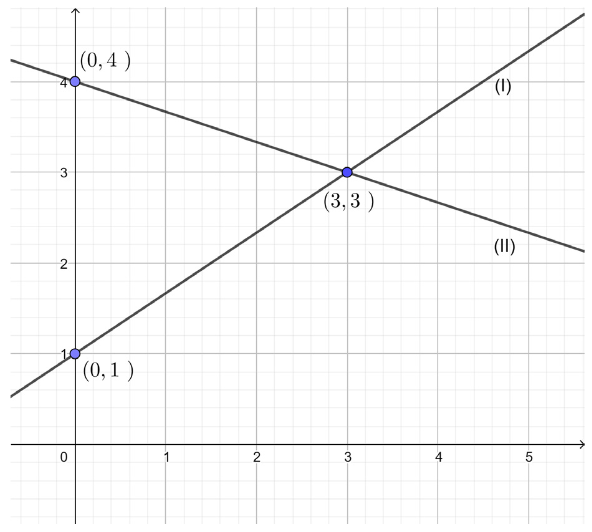
\includegraphics[scale=0.5]{LGS-graphische-lösung.png}
\end{figure}


%---------------------------------------------------------
\noaddpoints
\question[\totalpoints] % Barth SE K4.2 A3
\addpoints
Céline muss das folgende Gleichungssystem lösen: \[\systeme{x+5y=3,x-3y=2}\]
\begin{parts}
	\part[1] Sie beschliesst, dass Additionsverfahren zu verwenden, weil sie beobachtet, dass $x$ in beiden Gleichungen den Koeffizient 1 hat. Sie fasst also den Plan die zweite Gleichung mit $-1$ zu multiplizieren und anschliessend beide Gleichungen zu addieren. Was genau wird sie dann erhalten?
	\part[3] Wie müsste Céline vorgehen, um im Additionsschritt die Variable $y$ zu eliminieren? Erkläre in Worten \textbf{und} berechne die Lösung des Gleichungssystems\footnote{Lösungen ohne Additionsverfahren haben einen Punkteabzug zur Folge.}.
\end{parts}

%---------------------------------------------------------
\noaddpoints
\question[\totalpoints] % Barth SE K4.2 A4
\addpoints
Max muss das folgende Gleichungssystem lösen: \[\systeme{2x+y=1,7x-y=2}\]
\begin{parts}
	\part[2] Er möchte sich in der Additionsmethode üben und fasst folgenden Plan: Er möchte die erste Gleichung mit 7 und die zweite Gleichung mit  2  multiplizieren. Danach will er die beiden Gleichungen addieren und damit die Variable x eliminieren. Funktioniert das? Begründe deine Antwort.
	\part[2] Löse das Gleichungssystem vollständig mit Hilfe des Additionsverfahren.
\end{parts}


%---------------------------------------------------------
\question[4] % Algebra 9/10 S84 A12a
Löse das folgende lineare Gleichungssystem mit einem Verfahren deiner Wahl.
\[\systeme{-2x+4y=4,-x+3y=4}\]


%---------------------------------------------------------
\question[4] %DMK Algebra A16e S67
Löse das folgende Gleichungssystem unter Verwendung des Einsetzungsverfahren.
\[\systeme{\frac{1}{4}x-\frac{5}{6}y=5,\frac{4}{5}x-y=11}\]
{\small\textbf{Bewertung:} Wird nicht das erwähnte Verfahren verwendet, wird die Aufgabe mit 0 Punkte bewertet.}

%---------------------------------------------------------
\question[5] % Barth Ü&A K4.3 A4a
Vereinfache das folgende lineare $3\times3$ Gleichungssystem auf ein einfacheres $2\times2$ System, in dem du die Gleichungen geeignet umformst. Du musst das Gleichungssystem nicht komplett auflösen.
\[\left\{\begin{matrix}5x-2y=8+2z\\z+2x=11-7y\\y=2.5x-z-4\end{matrix}\right.\]


%---------------------------------------------------------
\question[5] % DMK Algebra 9/10 S84 A17c
Vereinfache das folgende lineare $3\times3$ Gleichungssystem auf ein einfacheres $2\times2$ System, in dem du die Gleichungen geeignet umformst und addierst. Du musst das Gleichungssystem nicht komplett lösen.
\[\systeme{7x-6y+5z=18,5x+3y-4z=28,8x+2y+3z=26}\]


%---------------------------------------------------------
\question[4]
Löse das folgende lineare $3\times3$ Gleichungssystem unter Verwendung eines geeigneten Verfahrens. \[\systeme{6x-y+z=12,-6y+z=1,x+3y+z=-3}\]


%---------------------------------------------------------
\question[4]
Löse das folgende lineare $3\times3$ Gleichungssystem unter Verwendung eines geeigneten Verfahrens. \[\systeme{2x-y+z=1,-x+2y=1,x+2y+z=5}\]


%---------------------------------------------------------
\question[4] %Barth Nachtest A4c
Löse das folgende lineare Gleichungssystem unter Verwendung eines geeigneten Verfahrens. Bemerke, $p$ ist hier ein Parameter. \[\left\{\begin{matrix}5x-3y=14p\\-x+5y=6p\end{matrix}\right.\]


%---------------------------------------------------------
\question[4] % DMK Algebra A15a S84
Bestimme die Lösungsmenge des folgenden linearen Gleichungssystems. Bemerke, $d$ ist hier ein Parameter.
\[\left\{\begin{matrix}x-y=d\\\frac{x-y}{2}+dx=d\end{matrix}\right.\]


%---------------------------------------------------------
\question[4] %DMK Algebra A9c S69
Löse das folgende lineare Gleichungssystem unter Verwendung eines geeigneten Verfahrens. Bemerke, $r$ ist hier ein Parameter. \[\left\{\begin{matrix}(r-1)x=r(1-x)\\r(r-x-y)=2x\end{matrix}\right.\]


%---------------------------------------------------------
\question[6] % KSWilli A15
Bauer Heiniger aus dem Toggenburg hält Schweine und Hühner. Insgesamt haben seine Tiere $594$ Beine. Die Anzahl der Hühner ist um $9$ grösser als die doppelte Anzahl Schweine. Wie viele Schweine und wie viele Hühner hält Bauer Heiniger?


%---------------------------------------------------------
\question[5] %KSWilli A16
Das Verkehrshaus in Luzern hat unterschiedliche Eintrittspreise für Erwachsene und Kinder. Herr und Frau Schmidiger zahlen mit ihren vier Kindern $36$ CHF Eintritt. Frau Vetter und ihre drei Kinder zahlen $23$ CHF. Was kostet der Eintritt für Erwachsene und Kinder?

%---------------------------------------------------------
\question[5] % Gauss-Verfahren
Löse das folgende lineare Gleichungssystem mit Hilfe des Gauss-Verfahrens.
\[\systeme{x-2y+5z=0,4x-4y+16z=6,-3x+8y-18z=-3}\]
{\small\textbf{Bewertung:} Wird nicht das erwähnte Verfahren verwendet, wird die Aufgabe mit 0 Punkte bewertet.}


\end{questions}
\end{document}